\documentclass[english,biblatex]{lni}
\usepackage{hyperref}
\usepackage[backend=biber]{biblatex}
\addbibresource{systems-engineering.bib}
\ExecuteBibliographyOptions{}
\graphicspath{{figures/}}
\DeclareGraphicsExtensions{.pdf,.jpeg,.jpg,.png}
\graphicspath{{figures/}}


\begin{document}

\title[Improving the Efficiency of Dislocality Constraints]{Improving the Efficiency of Dislocality Constraints for an Automated Software Mapping in Safety-Critical Systems}
%%% \subtitle{Untertitel / Subtitle} % if needed
\author[Robert Hilbrich \and Michael Behrisch]
{Robert Hilbrich\footnote{German Aerospace Center (DLR), Rutherfordstr. 2, 12489 Berlin,
Germany \email{robert.hilbrich@dlr.de}} \and
Michael Behrisch\footnote{German Aerospace Center (DLR), Rutherfordstr. 2, 12489 Berlin,
Germany \email{michael.behrisch@dlr.de}}}
\startpage{11} % Beginn der Seitenzählung für diesen Beitrag / Start page
%\editor{Herausgeber et al.} % Names of Editors
\booktitle{SE’18: Software Engineering-Tagung der Gesellschaft für Informatik (GI)} 
\year{2018}

\startpage{1}

\maketitle

\begin{abstract}
This is a brief overview of the paper, which should be 70 to 150 words long and
include the most relevant points. This has to be a single paragraph.
\end{abstract}


\begin{keywords}
Keyword1 \and Keyword2
\end{keywords}


\section{Introduction}

Engineering complex and safety-critical systems, such as flight control systems aboard an airplane, is still challenging and costly.
Despite recent advancements in our model-based tool suites and engineering methods, the design of these systems still bears risk and uncertainties with regard to its outcome.
The formalization and automation of crucial engineering tasks appears to be a promising approach to tackle these challenges~\cite{Chapman2007}.
Systems in these areas are engineered to implement a complex interplay between mechanical elements, electronic components, as well as (embedded) software.
Therefore, their design has to mirror this interplay and requires the development of a hardware and software architecture.

In practice, these architectures can often be developed independent of each other, but their integration in the final system requires a \emph{link} between the software components and their hardware resources.     
This \emph{link} is referred to as a \emph{deployment} of the software components.
Constructing a deployment requires the systems engineer to \emph{map} software components to resources and to \emph{schedule} the access to shared resources.
Therefore, mapping refers to a \emph{spatial allocation}, while scheduling refers to a \emph{temporal allocation} of software components.

The construction of a deployment is an engineering task, which not only affects the fulfillment of functional requirements by providing the necessary, but also affects the satisfaction of non-functional requirements, such as safety and reliability.
Redundancy and fault tolerance can only be achieved, if critical software components are deployed accordingly.

The construction of a deployment is a very elaborate task with zero tolerance for errors as they may jeopardize the correctness of the system.
At the same time, it requires a detailed understanding of the requirements of all software components and the capabilities of all hardware resources in the system.
Due to the sensitivity and complexity of this task, its formalization and automation is a valuable research goal.

\section{Automated Construction of Deployments}

In order to achieve an automated construction of a deployment and to argue its correctness, a formalization of the mapping problem is required.
For smaller mapping problems, this has been successfully achieved based on Linear Integer Programming~\cite{Damm2006, Kugele2009}, SMT-based solvers~\cite{Voss2013} or evolutionary algorithms~\cite{White2011}.
However, these approaches reach their limits when larger, real-world mapping problems with limited gradient information to guide a search process are considered.

The authors instead chose to transform a mapping problem into a semantically equivalent \emph{Constraint Satisfaction Problem (CSP)}~\cite{Apt2003,Dechter2003} and solve this CSP with \emph{Constraint Programming} techniques~\cite{Rossi2006,Prudhomme2016}.
The advantages of using Constraint Programming in comparison to other techniques lie in the availability of powerful modeling elements, such as an \textsc{allDifferent} constraint, and the ease with which custom search heuristics can be implemented.

\subsection{Constraint Satisfaction Problems}
Constraint Programming refers to a set of techniques in artificial intelligence and operations research.
These techniques assist in finding solutions for problems based on variables, which are affected by constraints.
Each constraint defines valid or invalid solutions for a subset of these variables.
In this paper, a subclass of constraint satisfaction problems is used to express mapping problems:  \emph{finite domain integer constraint satisfaction problems} in which each variable has a finite integer domain.
Solutions for this problem class can be obtained by applying a combination of \emph{search} techniques -- including backtracking -- and constraint \emph{propagation} techniques for value elimination.

To illustrate the modeling approach of Constraint Satisfaction Problems, consider the well-known \emph{Map Coloring} problem as an example.
This problem asks, whether it is possible to color a map with only four colors in such a way, that neighboring countries have different colors.
It can be formulated as a CSP by assigning an integer variable $x_i$ for each country with the index $i$.
The domain of each variable corresponds to the four colors: $D_{x_i}=\{0,1,2,3\}$.
In order to model the restrictions of this problem, a constraint is added for each pair of adjacent countries.
If country $x_i$ is adjacent to country $x_j$, then $x_i \neq x_j$ is required.
The search algorithm is now responsible to select a variable and test a value of its domain.
Assuming a simple ``first variable, first value'' strategy, the variable $x_0$ would be chosen and set to the value $0$ as a test.
This would be \emph{propagated} to all variables which are directly linked to $x_0$ by a constraint, so that the value $0$ gets removed from their domains.
This removal may lead to other value removals in indirectly linked variables and is processed until a fix point is reached.
If a contradiction is encountered or the domain of a variable becomes empty, \emph{backtracking} is initiated, so that the next value of the variable $x_0$ is tested.
Otherwise, the search algorithm continues with the next uninstantiated variable.

This example also shows, that the propagation of the \textsc{NotEqual} constraint is \emph{weak}, because it affects only two variables and invalidates only 4 out of the 16 possible value combinations between two variables.

\subsection{Toolsuite ASSIST}
As a proof of concept for the ongoing research toward an automated construction of deployments based on Constraint Satisfaction Problems, the toolsuite \emph{Architecture Synthesis for Safety-Critical Systems (ASSIST)}~\cite{ASSIST} was developed by the authors.
It is open source and uses the constraint solver \emph{Choco}~\cite{Prudhomme2016} internally.
ASSIST (see Figure~\ref{tool}) allows a systems engineer to automatically construct and optimize mappings and schedules based on textual specifications of the

\begin{itemize}
\item software components and hardware resources,
\item constraints for valid/invalid assignments (\textit{dislocality}, \textit{dissimilarity}, \textit{colocality}) and 
\item optimization goals.
\end{itemize}

The textual specifications in ASSIST conform to a domain-specific language which allows to hide the intricacies of a formal specification.
Using a domain-specific language is expedient to enable systems engineers without a formal education in computer science to precisely specify a deployment problem.

\begin{figure}[!t]
\centering
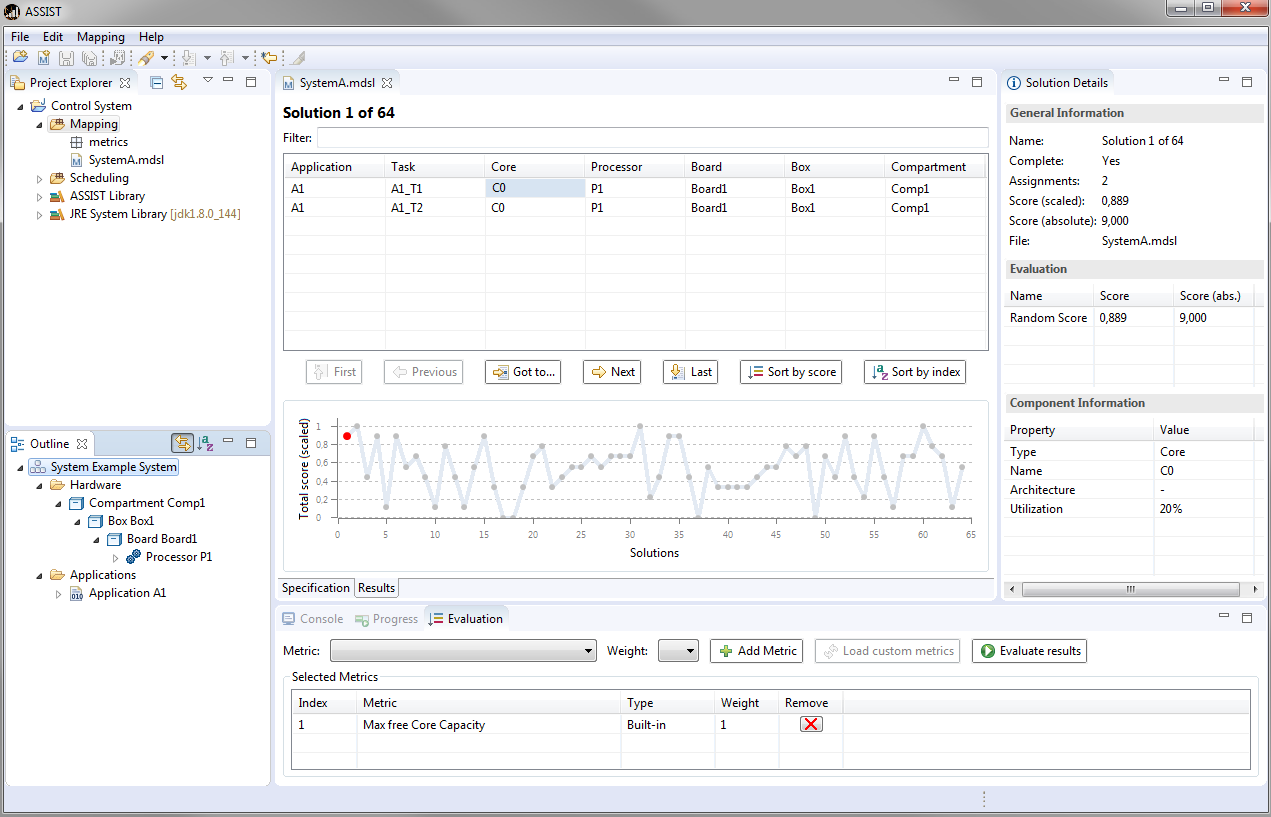
\includegraphics[width=\textwidth]{assist-screenshot}
\caption{Screenshot of ASSIST with a specification for a control system}
\label{tool}
\end{figure}

\section{Ensuring Redundancy by Requiring Dislocality}

\begin{itemize}
\item In order to ensure a reliability / redundancy work properly - it is essential to ensure is differences
\item Differences in the deployment of redundant software components to make sure that the errors do not appear in the same manner at the same location (zonal effects)
\item Dislocality is a typical constraint in ASSIST to express these differences
\item Simple Modeling approach for a CSP (location variables)
\item Use allDiffererent constraint - straight forward
\item Reality: AllDifferent for List of Lists
\item Example to describe the differences
\end{itemize}

\section{Modeling Advanced Dislocality Constraints}

\begin{itemize}
\item Based on available tools - one option is the recursive approach
\item Implementation is straight forward, but it requires a lot of constraints - slow in practice
\item Another option is to react on instantiation only and remove unwanted solutions - weak in propagation
\item Last Option is to combine inst-only approach with int-values union and alldifferent
\end{itemize}

\section{Experiments}

\begin{itemize}
\item Synthetic example generator 
\item 10/20 Examples were generated with a parameter domain ...
\item Search with the same strategies DomWD, minValueFirst
\item iMac 5k, 64 GB RAM, Choco 4.0.6
\end{itemize}

\section{Results}

\begin{itemize}
\item Show results for var count, constraint count
\item Show results for resolution time
\item Show results for backtracks and fails
\end{itemize}

\section{Conclusions}

I am a summary - what shall i put here?

\printbibliography[heading=bibintoc]

\end{document}

%%% Local Variables: 
%%% mode: latex
%%% TeX-master: "paper"
%%% ispell-check-comments: exclusive
%%% ispell-local-dictionary: "english"
%%% End:
